\documentclass[12pt]{article}
\usepackage{graphicx} % Required for inserting images
\usepackage{enumitem}
\usepackage{amsmath}
\usepackage{gvv-book}
\usepackage{gvv}

\title{\textbf{4.5.6}}
\author{\textbf{EE25BTECH11004 - Aditya Appana}}
\date{September 12, 2025}

\begin{document}

\maketitle

\section*{Question}
Find the equations of the line that passes through the point (3,0,1) and parallel to the
planes $x + 2y = 0$ and $3y$ $-$ $z = 0$.

\section*{Solution}

We know that the normal form of a plane is $\vec{n}^T\vec{x} = 0$ \\
The plane $x + 2y = 0$ can be expressed in vector form as:
\begin{align}
    \myvec{1\\2\\0}^T\vec{x} = 0
\end{align} 

therefore, \begin{align}\vec{n}_1 = \myvec{1\\2\\0}\end{align} \\
The plane $3y$ $-$ $z=0$ can be expressed in vector form as:

\begin{align}
    \myvec{0 \\ 3 \\-1}^T\vec{x} = 0
\end{align}

therefore, \begin{align}\vec{n}_2 = \myvec{0\\3\\-1} \end{align}

The vector parallel to both planes will be perpendicular to the normal vectors of both planes. Therefore it can be expressed as
\begin{align} \vec{n}_1 \times \vec{n}_2 \end{align}

To calculate the cross product of the two vectors \vec{a} and \vec{b}, we use the following determinant:
\begin{align}
\myvec{|\vec{A_{11}} \vec{B_{23}}| \\ |\vec{A_{11}}   \vec{B_{23}}| \\ |\vec{A_{11}} \vec{B_{23}}| }
\end{align}
Where \vec{X_{ij}} = \myvec{$x_i$ \\ $x_j$}. \\

Expanding the determinants, we get: \begin{align}
\myvec{ ((-2) - 0) \\ (1-0)  \\ (3-0))} = \myvec{-2\\1\\3} \end{align}\\ 

Since the line passes through (3,0,1), the line can therefore be expressed as: \\
\begin{align}
\frac{x-3}{-2} = \frac{y}{1} = \frac{z-1}{3}
\end{align} 

\begin{figure}[H]
    \centering
    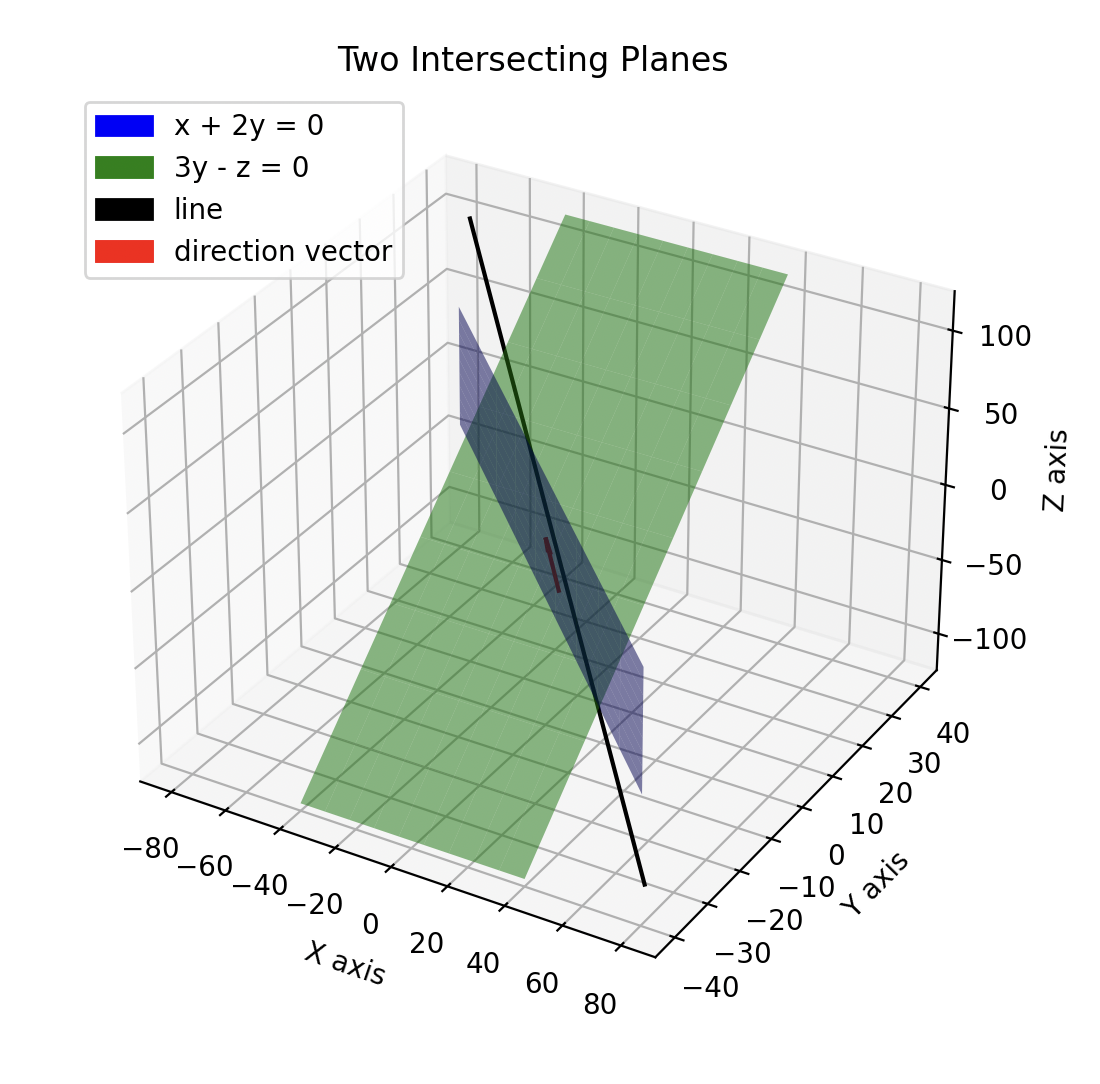
\includegraphics[width=0.9\columnwidth]{Figs/Plot7.png}
    \caption{Plot}
    \label{fig:placeholder}
\end{figure}



\end{document}